%%%%
\documentclass[12pt,a4paper]{report}
% o article, book, ...

% TODO inserire vari packages (todonotes, ecc.)

%%%%%%%%%%%%%%%%%%%%%%%%%%%%%%%%%%%%%%%%%%%%%%%%%%%%%%
% packages...
\usepackage[utf8]{inputenc}
\usepackage[english,italian]{babel}
\usepackage[hyphens]{url}
\usepackage{csquotes}
% Per generare il file PDF aderente alle specifiche PDF/A-1b. Verificarne poi la validità.
%\usepackage[a-1b]{pdfx}

\usepackage{hyperref}
\usepackage{graphicx}
\graphicspath{ {Img/} }
\usepackage{lipsum}% Per inserire testo a caso in attesa di realizzare i capitoli
\usepackage{listings}
\usepackage{epigraph} % per le frasi inizio capitolo
\usepackage{fancyhdr}
\usepackage{refcheck}


\lstset{
	% 	language=bash
	frame=single,
	breaklines=true,
	postbreak=\raisebox{0ex}[0ex][0ex]{\ensuremath{\color{red}\hookrightarrow\space}},
	basicstyle=\ttfamily\footnotesize
}
%--- BIBIOGRAFIA
\usepackage[ backend=biber, style=alphabetic,
%citestyle=authoryear 
]{biblatex}

\addbibresource{Biblio.bib}
%---

\usepackage[colorinlistoftodos]{todonotes}
%\usepackage[disable]{todonotes}

%%%%%%%%%%%%%%%%%%%%%%%%%%%%%%%%%%%%%%%%%%%%%%%%%%%%%
\begin{document}

% Frontespizio
\begin{titlepage}
\begin{center}

\includegraphics[width=\textwidth]{Img/Logo.jpg}\\
{\large{\bf Corso di Laurea Informatica}}
\end{center}
\vspace{12mm}
\begin{center}
{\huge{\bf TITOLO}}\\
\vspace{4mm}
{\huge{\bf TITOLO}}\\
\vspace{4mm}
{\huge{\bf TITOLO}}\\
\end{center}
\vspace{12mm}
\begin{flushleft}
{\large{\bf Relatore:}}
{\large{Trentini Andrea}}\\
\vspace{4mm}
{\large{\bf Correlatore:}}
{\large{Carraturo Alexjan}}\\
\end{flushleft}
\vspace{12mm}
\begin{flushright}
{\large{\bf Tesi di Laurea di:}}
{\large{Bianchessi Mattia}}\\
{\large{\bf Matr. 931455}}\\
\end{flushright}
\vspace{4mm}
\begin{center}
{\large{\bf Anno Accademico xxxxxxxx}}
\end{center}
\end{titlepage}

%%%%%%%%%%
% TODO
%%%%%%%%%%
\listoftodos

%%%%%%%%
\chapter*{Introduzione}

Introduzione 
\todo{Introduzione \ldots}



\tableofcontents
\listoffigures
\listoftables

% o sections (dipende dal documentclass)

\chapter{RISC-V}
\todo{Rileggi/Correggi capitolo 1: RISC-V \ldots} 

% OUTLINE CH 1
%	definizione di computer \\
%	presentazione progetto \\
%	applicazione dalla nascita ad oggi  \\


\section{Dal codice alle istruzioni}
\begin{quote}
\textbf{Computer}  :
Apparecchio elettronico in grado di svolgere operazioni matematiche e logiche e di memorizzare informazioni a una velocità e in una quantità superiori a quelle di cui è comunemente capace il cervello umano; nelle sue componenti materiali ( hardware ) [..] e da un insieme di circuiti e di dispositivi sui quali si svolgono le funzioni di memoria, di elaborazione e di controllo, che avvengono grazie a programmi contenenti istruzioni ( software ); tali programmi sono basati su un sistema di computazione binario e sono scritti in vari linguaggi di programmazione;
\cite{DefinizioneComputer}
\end{quote}

Essere in grado di programmare significa essere in grado di scrivere un elenco di istruzioni interpretabili dal computer ed eseguibili. Il linguaggio scelto, che sia di alto livello o di basso livello,  deve essere tradotto in linguaggio macchina in questo modo puo essere eseguito dal nostro computer. Questo processo di chiama processo di compilazione mediante il quale il codice , scritto in linguaggio leggibile (human readeable) viene tradotto in codice sorgente che verrà poi sottoposto a determinate verifiche per poter essere approvato e trasformato in codice oggetto e poi file eseguibile.\\
All' interno del computer la componente che si occupa dell' esecuzione del codice è la CPU che,  leggendo le istruzioni tradotte dal codice (scritto e poi compilato) esegue delle operazioni specifiche. Come è normale pensare esistono differenti processori , differenti per frequenza di clock, memoria di cache, architettura interna  o tensione di alimentazione. Quindi il è necessario che il codice si chiaro e capibile per un determinato processore. \\

Un'Instruction Set Architecture (ISA) definisce il modello astratto di un computer ovvero come la CPU controlla hardware e software., specificando sia ciò che il processore è in grado di fare sia come viene fatto.

L'ISA fornisce l'unico modo attraverso il quale un utente è in grado di interagire con l'hardware. Può essere visto come un manuale del programmatore perché è la parte della macchina visibile al programmatore in linguaggio macchina,  allo scrittore del compilatore e al programmatore dell'applicazione.
L'ISA, inoltre, definisce i tipi di dati supportati, i registri, il modo in cui l'hardware gestisce la memoria principale. 

In informatica esistono due tipi popolari di architetture basate sul set di istruzioni. Si tratta di CISC (Complex Instruction Set Computing) e RISC (Reduced Instruction Set Computing).


Il primo approccio consiste in un ISA formata da un set di istruzioni in grado di eseguire operazioni complesse tramite una singola istruzione. Contrariamente il secondo approccio snellisce il set di istruzioni che porta ad avere un architettura più semplice e lineare.

\section{progetto RISC-V}
Il RISC-V è un progetto open source basato su un architettura di tipo RISC. Il progetto iniziato nel 2010 all'Università della California, Berkeley. In origine Prof. Krste Asanoviće e alcuni studenti (Yunsup Lee e Andrew Waterman) svilupparono un ISA per scopi didattici, inizialmente solo progettata e successivamente, dopo dei finanziamenti, prodotta. Il primo workshop risale al 2015 e al lancio il progetto contava 36 membri fondatori.

L'interesse per RISC-V non è dovuto all' architettura RISC o alla tecnologia rivoluzionaria ma il punto fondamentale è che RISC-V è uno standard libero che consente a chiunque di sviluppare in modo libero il proprio hardware per seguire il software.\\

Dopo il lancio il progetto fu studiato e utilizzato da molte realtà , come ad esempio in DARPA e Linux Foundation ,  e fu per questo che si fece conoscere molto presto al mondo.  Ora Il progetto RISC-V presenta numerose partnership con aziende e una community sparsa per tutto  il mondo.



\chapter{ISA RISC-V}
\section{ISA Overview}
\section{ISA Base}
\section{ISA Ext}

\chapter{Compilatori}

\todo{Rileggi capitolo\ldots}

\section{Descrizione}
Un compilatore è un programma che trasforma il codice sorgente scritto in un determinato linguaggio di programmazione,  in un altro linguaggio informatico (codice target). Il motivo più comune per trasformare il codice sorgente è creare un programma eseguibile. Il linguaggio attraversa diverse fasi prima di diventare il codice target. La prima attivita è l' analisi lessicale dove il programma viene analizzato parola per parola e genera dei token. La seconda attivita è l analisi sintattica dove viene controllata la correttezza formale del programma. In questa fase i token precedentemente generati vengono analizzati e utilizzati per generare una struttura ad albero che nella fase di analisi semantica viene analizzato per verificare la correttezza delle espressioni scritte.  Infine viene generato il codice target.  Alcuni compilatori prevedono un ulteriore fase la fase di ottimizzazione dove il codice viene ottimizzato 

\begin{figure}
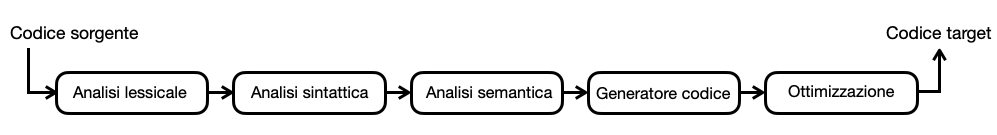
\includegraphics[width = \textwidth]{SchemaCompilatore.png}
\caption{Schema meccanismo di compilazione}
\end{figure}


Qualsiasi programma scritto in un linguaggio di programmazione di alto livello deve essere tradotto in codice oggetto prima di poter essere eseguito, quindi tutti i programmatori che utilizzano tale linguaggio utilizzano un compilatore o un interprete. I miglioramenti a un compilatore possono portare a un gran numero di funzionalità migliorate nei programmi eseguibili.

\section{Storia}
Il primo compilatore teorico fu pensato da Corrado Böhm che nel 1951 che lo sviluppò per la sua tesi di dottorato . Il primo compilatore implementato è stato scritto da Grace Hopper , coniando il termine "compilatore". Il primo compilatore , chiamato sistema A-0,  funzionava come caricatore o linker , non come i moderni compilatori. E' importante menzionare che una versione successiva (la versione A-2 datata 1953)fu il primo software libero e open source della storia dell'informatica. \\

Il primo compilatore ALGOL 58 fu completato alla fine del 1958 da Friedrich L. Bauer , Hermann Bottenbruch, Heinz Rutishauser e Klaus Samelson per il computer Z22 . 
Nel 1960, un compilatore Fortran esteso, ALTAC, era disponibile sulla Philco 2000, quindi è probabile che un programma Fortran sia stato compilato per le architetture di computer IBM e Philco a metà del 1960.  Il primo linguaggio di alto livello multipiattaforma noto è stato COBOL. 

Come qualsiasi altro software, ci sono vantaggi nell'implementare un compilatore in un linguaggio di alto livello. In particolare, un compilatore può essere self-hosted , ovvero scritto nel linguaggio di programmazione che compila. Il sopracitato compilatore di Böhm è un compilatore self-hosted. Il suo compilatore, oltre ad essere completo, fu il primo definito con il proprio linguaggio.
Oltre a quel compilatore possiamo citare il Navy Electronics Laboratory International ALGOL Compiler (NELIAC) o il Lisp.\\

Come durante una comunicazione verbale anche i programmi hanno una propria grammatica con regole queste vengono analizzate da un parser, generato da un generatore, ha lo scopo di analizzare come è scritto il programma e generare i token associati. Un primo progetto risale al 1960 come progetto dell università di Università di Manchester, non è da considerare un compilatore moderno ma un buon punto per la costruzione e per l ideazione del sistema Unix nel 1969 da parte di Ken Thompson.\\

\section{Cross-compilazione}
Un compilatore incrociato è un compilatore in grado di creare codice eseguibile per una piattaforma diversa da quella su cui è in esecuzione il compilatore. Ad esempio, un compilatore che viene eseguito su un PC ma genera codice che viene eseguito su uno smartphone Android è un compilatore incrociato.

Un compilatore incrociato è utile per compilare codice per più piattaforme da un host di sviluppo. La compilazione diretta sulla piattaforma di destinazione potrebbe non essere fattibile, ad esempio su sistemi embedded con risorse informatiche limitate.

\section{Compilatori moderni}

gcc, LLVM, AMR


\chapter{BenchMarking}
\section{Descrizione board}

La scheda di sviluppo utilizzata è  D1-H Nezha basata sul design del chip Allwinner D1-H. La board integra una CPU Ali Pingtou Ge RISC-V C906, con clock a 1 GHz, supporta il kernel Linux standard, supporta  2G DDR3, 258 MB di spin-nand, WiFi/Bluetooth connessione, con interfacce audio e video,  può essere collegato a varie periferiche, interfaccia MIPI-DSI+TP integrata, interfaccia scheda SD,interfaccia HDMI, interfaccia scheda figlia microfono, interfaccia auricolari da 3,5 mm , interfaccia Gigabit Ethernet, USB HOST, interfaccia di tipo C, interfaccia di debug UART, array di pin a 40 pin.

\begin{figure}
\includegraphics[width = \textwidth]{D1H-BoardTopView.png}
\caption{Board vista dall' alto}

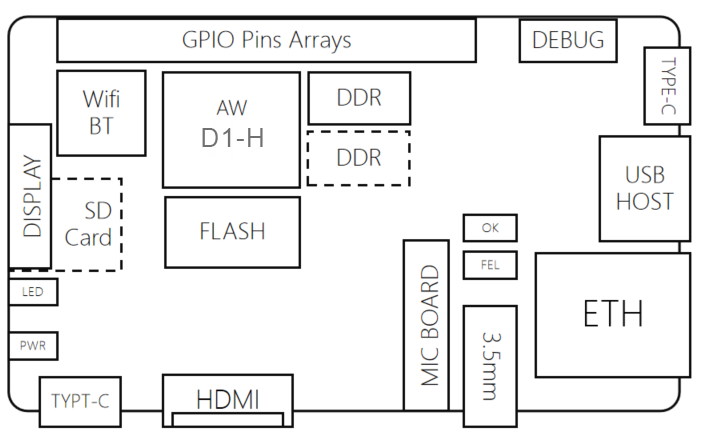
\includegraphics[width = \textwidth]{D1H-BoardBlockView.png}
\caption{Schema a blocchi della scheda di sviluppo}
\end{figure}

\vspace{2cm}
\begin{table}
\centering
\begin{tabular}{|r|c|}
\hline
CPU & Allwinner D1-H \\
\hline
Clock & 1GHz\\
\hline
DRAM & DDR3 2GB\\
\hline
Memoria & 256MB  spin-nand integrato\\
\hline 
Supporto memoria & USB e  SD\\
\hline
Rete & Gigabit Ethernet,  2.4G WiFi e Bluetooth , antenna integrata\\
\hline
Display & MIPI-DSI + TP, HDMI, SPI \\
\hline
Audio & jack per cuffie da 3,5 mm\\
\hline
Tasti & FEL, LRADC OK\\
\hline
Luci &  alimentazione, LED tricolore\\
\hline
DEBUG & UART, USB ADB\\
\hline
USB & USB , USB OTG, USB2.0\\
\hline
PIN & array di pin 40\\
\hline
Alimentazione & USB-C  5V-2A\\
\hline
Dimensioni & lunghezza 85 mm * larghezza 56 mm * spessore 1,7 mm\\
\hline

\end{tabular}
\caption{Caratteristiche della board}
\end{table}

\section{Ulteriori informazioni}
BAD TITLE !!!\\
info ambiente di sviluppo
\section{presentazione programmi}

\chapter{Comparativa}
\section{analisi codice assembly}
\section{Confronto Sorting}

\chapter{Progetti }

\chapter{Conclusione}

%\addcontentsline{toc}{chapter}{Bibliografia}

\printbibliography

\end{document}
